%!TEX root = ../var.tex

\subsection{Сферическое распределение}

\begin{definition}
Пусть случайные величины $\xi_1 , \ldots , \xi_n$ независимы и одинаково распределены по нормальному закону распределения
%
$$f_{\xi_i}(x_i) = \frac{1}{\sqrt{2\pi} \sigma} e^{-x^2_i/2\sigma^2},$$
%
то есть $a_i = 0$ и $\sigma_i = \sigma$ для всех 
%
$i = 1, \ldots , n.$ 
%
Тогда распределение случайного вектора $\xi = (\xi_1 , \ldots , \xi_n )$ называется нормальным сферическим распределением или проще сферическим распределением.
\end{definition}

\begin{lemma}
 Плотность вероятности сферического распределения есть
$$f_{\xi} (x_1 , \ldots , x_n ) = \frac{1}{(2\pi)^{n/2}\sigma^n} e^{-\frac{1}{2\sigma^2}(x_1^1 + \ldots + x^2_n)}$$
 \end{lemma} 

 \begin{proof}
 Это утверждение очевидно следует из 27.1 и 15.6.2).
 \end{proof}

\begin{zam}
Так как поверхности равной вероятности, то есть
$f_{\xi} (x_1 , \ldots , x_n ) = const$,
являются концентрическими $(n - 1)$ --мерными сферами $x^2_1 + \ldots + x^2_n = R^2$ 
с центром в начале координат, то сферическое распределение инвариантно относительно любого ортогонального преобразования
%
$A : \mathbb{R}^n \to \mathbb{R}^n$. 
%
То есть, если $\eta = A \cdot \xi$, то 
%
$f_{\eta}(x_1 , \ldots , x_n) = f_{\xi} (x_1 , \ldots , x_n )$,
%
где через $A$ обозначена ортогональная матрица.

Положим в сферическом распределении $\sigma = 1$, получим плотность вероятности

$$f_{\xi}(x_1, \ldots, x_n) = \frac{1}{(2\pi)^{n/2}}e^{-\frac{1}{2}(x_1^2 + \ldots + x_n^2)} $$

и назовём её плотностью вероятности стандартного сферического распределения.
\end{zam}

\subsection{$\chi$-- и $\chi^2$-- распределения}

\begin{definition}
Пусть случайные величины $\xi_1 , \ldots , \xi_n$ независимы и одинаково распределены по стандартному нормальному закону распределения. Случайные величины

$$\chi = \sqrt{\xi_1^2 +\ldots + \xi_n^2 }$$

и

$$\chi^2 = \xi_1^2 + \ldots + \xi_n^2$$

называются соответственно $\chi-$ и $\chi^2$ -распределениями с $n$ степенями свободы.

Наша ближайшая задача найти их плотности вероятности $f_{\chi} (x)$ и $f_{\chi^2} (x)$.
\end{definition}

\begin{figure}[H]
	\centering
	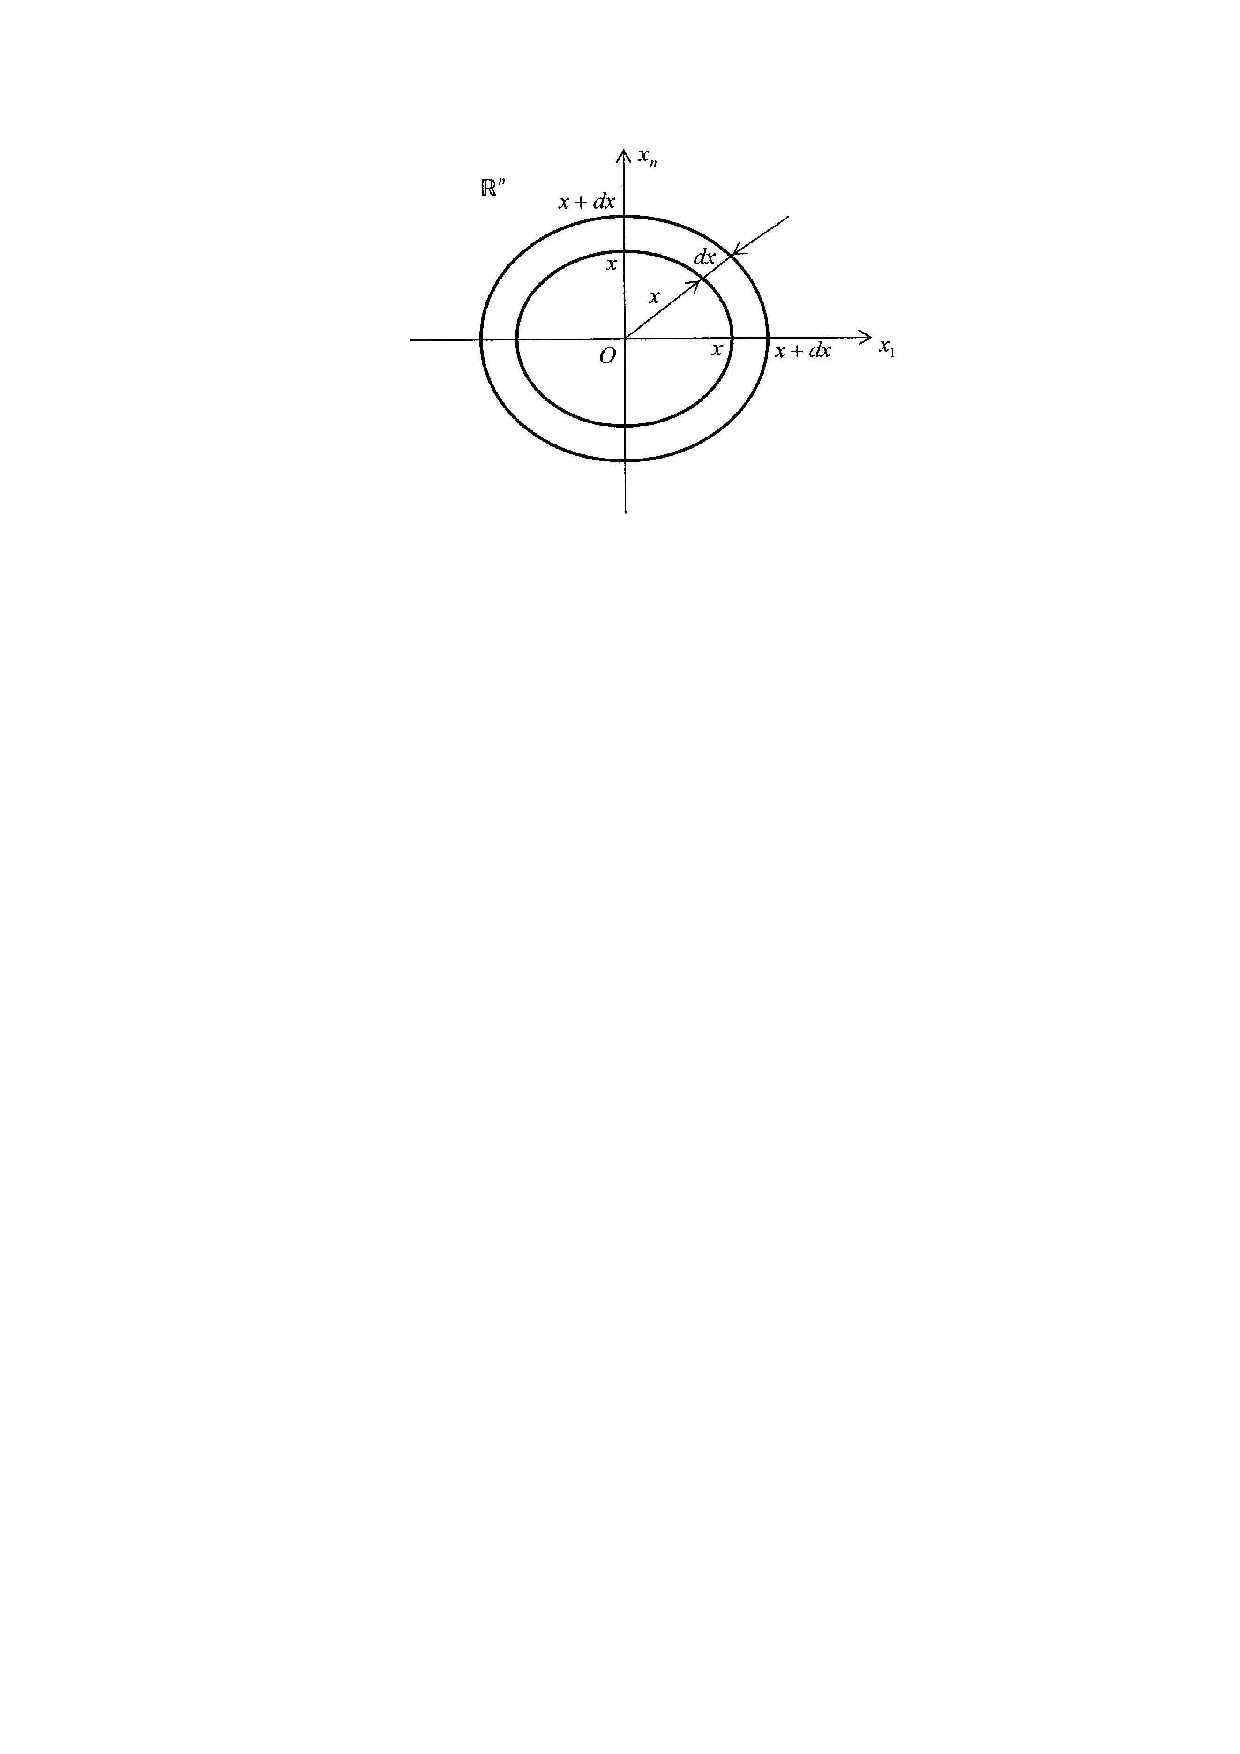
\includegraphics[]{pic/pic26}
	\caption{К вычислению плотности $\chi$-распределения}
	\label{fig26}
\end{figure}

\begin{theorem}
Плотность вероятности $\chi$-распределения задаётся по
формуле
$$f_{\chi} (x) = \frac{x^{n-1}}{2^{\frac{n}{2}-1}\Gamma(\frac{n}{2})} e^{-\frac{1}{2}x^2}, x\geqslant 0$$
где $\Gamma (x)$— гамма-функция.
\end{theorem}

\begin{proof}
Вероятность события $\{x < \chi < x + dx \}$ можно вычислить, интегрируя плотность вероятности $f_{\xi} (x_1 , \ldots , x_n )$ стандартного сферического распределения по $n$-мерному сферическому слою радиуса $x$ и толщины $dx$
(см. рис. 26).

$$ P(x < \chi < x + dx) = \dotsint\limits_{x<\sqrt{x_1^2 + \ldots + x_n^2}<x + dx} f_{\xi} (x_1 , \ldots , x_n ) dx_1 \ldots dx_n .$$

Откуда получаем

\begin{gather*}
f_{\xi} (x) = 
\frac{\P(x < \chi < x+dx)}{dx} = 
%
\dotsint\limits_{\sqrt{x_1^2 + \ldots + x_n^2} = x} 
f_{\xi}(x_1, \ldots, x_n)dx_1 \ldots dx_n = \\=
%
\frac{1}{(2\pi)^{n/2}} 
\dotsint\limits_{\sqrt{x_1^2 + \ldots + x_n^2} = x} e^{-\frac{1}{2}(x_1^2 + \ldots + x_n^2)}dx_1 \ldots dx_n = \\=
%
\frac{1}{(2\pi)^{n/2}}e^{-\frac{1}{2}x^2} 
\dotsint\limits_{\sqrt{x_1^2 + \ldots + x_n^2} = x} dx_1 \ldots dx_n = Cx^{n-1}e^{-\frac{1}{2}x^2}
\end{gather*}

где последнее равенство справедливо потому, что площадь $(n - 1)$-мерной сферы радиуса $x$ пропорциональна $x^{n-1}$ . Чтобы найти константу $C$, воспользуемся свойством плотности $\int\limits_0^{\infty} f_{\chi} (x) dx = 1$, откуда получаем

$$C\int\limits_0^{\infty}x^{n-1}e^{-\frac{1}{2}x^2}dx = 2^{\frac{n}{2}-1} \Gamma(\frac{n}{2})C = 1$$

откуда и следует требуемый результат.
\end{proof}

\begin{theorem}
Плотность $f_{\chi^2} (x)$ случайной величины $\chi^2$ есть

$$ f_{\chi^2} (x) = \frac{x^{\frac{n}{2}-1}}{2^{\frac{n}{2}} \Gamma (\frac{n}{2})}e^{-\frac{x}{2}}, \quad x \geq 0$$ 
\end{theorem}

\begin{proof}
Ясно, что случайные величины $\chi$ и $\chi^2$ связаны функцией $g(x) = x^2$ . Поэтому по теор. 14.2, находим, что
$$f_{\chi^2} (x) = |(g^{-1}(x))'| \cdot f_{\chi}(g^{-1}(x)) = \frac{1}{2\sqrt{x}}f_{\chi}(\sqrt{x}) = \frac{x^{\frac{n}{2}-1}}{2^{\frac{n}{2}} \Gamma(\frac{n}{2})} e^{-\frac{x}{2}}, \quad x \geq 0$$ 
 \end{proof} 

 \begin{zam}
Заметим, что $\chi^2$ -распределение с двумя степенями
свободы $(n = 2)$ является показательным распределением 12.7 с параметром $\lambda = 1/2$ и с плотностью вероятности $\frac{1}{2}e^{-\frac{x}{2}}, x \geq 0$. А $\chi$-распределение с тремя степенями свободы $(n = 3)$ называется распределением Максвелла и описывает в кинетической теории газов распределение модуля скорости
частиц в состоянии термодинамического равновесия.
 \end{zam}

\subsection{О распределении Стьюдента}

\begin{zam}
Этот пункт имеет информативный характер. Распределение Стьюдента\footnote{Стьюдент — псевдоним английского химика и статистика Вильяма Госсета (William Sealy Gosset, 1876
— 1937). По окончании университета был (с 1899) младшим управляющим пивоваренной компании в Дублине. В то время в совете директоров компании уже понимали важность методов
теории вероятностей и статистики для массового производства и направили Госсета на стажировку в
Лондонский университет для изучения статистики. Вскоре Госсет получил теоретические результаты в
статистике, которые оказались важными для пивоварения и которые он хотел опубликовать. В компании
не возражали против его публикаций, однако совет директоров хотел, чтобы конкуренты как можно
дольше не знали о применении статистики на пивоварне. Это объясняет появление псевдонима Стьюдент.} часто возникает в прикладных задачах математической статистики. Пусть случайные величины $\xi_0 , \xi_1 , \ldots , \xi_n$ независимы и одинаково распределены по стандартному нормальному закону распределения

$$f_{\xi_i} (x_i) = \frac{1}{\sqrt{2\pi}}e^{{-x^2_i/2}}$$

для всех $i = 0, 1, \ldots , n$. Тогда случайная величина

$$\tau_n = \frac{\xi_0}{\sqrt{\frac{1}{n}(\xi_1^2 + \ldots + \xi_n^2)}}$$

называется отношением Стьюдента, её распределение называется распределением Стьюдента с $n$ степенями свободы. Формула плотности вероятности $\tau_n$ имеет вид

$$f_{\tau_n}(x) = \frac{\Gamma(\frac{n+1}{2})}{\sqrt{n\pi}\Gamma(\frac{n}{2})} \left(1 + \frac{x^2}{n} \right)^{-\frac{n+1}{2}}, \quad -\infty < x < \infty$$
\end{zam} 

\begin{zam}
Легко проверить, что последовательность отношений Стьюдента $\{ \tau_n\}^{\infty}_{n=1}$ слабо сходится к стандартному нормальному распределению, то есть

$$\lim\limits_{n \to \infty} f_{\tau_n}(x) = \frac{1}{\sqrt{2\pi}}e^{-\frac{x^2}{2}}$$
\end{zam} 